\documentclass[hyperref={bookmarks=false},aspectratio=169]{beamer}
\usepackage{hyperref,ragged2e,amsmath,amssymb,url,bm}
\usepackage{graphicx,booktabs,array}
\usepackage{tikz}
\usetikzlibrary{arrows.meta,positioning,calc,shapes.geometric,decorations.pathreplacing,matrix}
\graphicspath{{crops/}}
\usetheme{Goettingen}
% --- Paleta: azul profundo, dorado y papiro crema ---
\definecolor{azul}{HTML}{15437C}
\definecolor{azuloscuro}{HTML}{0B1F3A}
\definecolor{celeste}{HTML}{5694D6}
\definecolor{dorado}{RGB}{196,154,60}
\definecolor{papiro}{RGB}{246,239,220}
\definecolor{gris}{RGB}{70,78,96}
\setbeamercolor{structure}{fg=azul}
\setbeamertemplate{sidebar canvas right}[vertical shading][top=azul,bottom=azuloscuro]
\setbeamercolor{title in sidebar}{fg=dorado}
\setbeamercolor{author in sidebar}{fg=papiro}
\setbeamercolor{section in sidebar}{fg=papiro}
\setbeamercolor{section in sidebar shaded}{fg=dorado!70!papiro}
\setbeamercolor{subsection in sidebar}{fg=papiro}
\setbeamercolor{subsection in sidebar shaded}{fg=dorado!70!papiro}
\let\raggedright\justifying
\setlength{\RaggedRightRightskip}{0pt plus 1fil}
\setbeamertemplate{background canvas}{
\includegraphics[width=\paperwidth,height=\paperheight]{papiro.jpg}}
\setbeamercolor{normal text}{fg=black!88!azuloscuro}
\setbeamercolor{frametitle}{fg=azul}
\setbeamerfont{frametitle}{series=\bfseries}
\setbeamertemplate{section in toc shaded}{\leavevmode{\color{gris}\inserttocsection}\par}
\setbeamercolor{title}{fg=azul}
\setbeamercolor{subtitle}{fg=gris}
\setbeamercolor{item projected}{bg=azul,fg=papiro}
\setbeamertemplate{itemize item}{\small\textcolor{dorado}{$\blacktriangleright$}}
\setbeamertemplate{navigation symbols}{}
% --- Español + hebreo + griego (XeLaTeX) ---
\usepackage[bidi=default]{babel}
\babelprovide[import,main]{spanish}
\babelprovide[import]{hebrew}
\babelprovide[import]{ancientgreek}
\babelfont[hebrew]{sf}[Path=fonts/, BoldFont=NotoHebrewSans-700.ttf]{NotoHebrewSans-400.ttf}
\babelfont[hebrew]{rm}[Path=fonts/, BoldFont=NotoHebrewSans-700.ttf]{NotoHebrewSans-400.ttf}
\babelfont[ancientgreek]{sf}[Path=fonts/]{GFSPorson.otf}
\babelfont[ancientgreek]{rm}[Path=fonts/]{GFSPorson.otf}
\newcommand{\heb}[1]{\mbox{\foreignlanguage{hebrew}{#1}}}
\newcommand{\grc}[1]{\foreignlanguage{ancientgreek}{#1}}
\newcommand{\SENOR}{S{\fontsize{0.78em}{1em}\selectfont EÑOR}}
% --- Citas (cuadro de un solo color), imágenes, referencias ---
\usepackage[most]{tcolorbox}
\newtcolorbox{cita}[1][]{enhanced, colback=azul!7!papiro, opacityback=0.85, colframe=azul,
  boxrule=0pt, leftrule=2.5pt, arc=0pt, left=6pt, right=6pt, top=4pt, bottom=4pt,
  before skip=4pt, after skip=6pt, fontupper=\small\itshape, #1}
\newcommand{\fuente}[1]{\par\hfill{\upshape\bfseries\footnotesize\textcolor{azul}{#1}}}
\makeatletter
\newcommand{\fotolado}[2]{%
  \begin{tikzpicture}[remember picture,overlay]
    \node[anchor=north east,inner sep=0pt] (foto) at ([xshift=-\beamer@sidebarwidth]current page.north east)
      {\includegraphics[height=\paperheight]{#1}};
    \node[anchor=south east,inner sep=2pt,text=papiro,fill=azuloscuro,fill opacity=0.6,text opacity=1,
      font=\fontsize{4.5}{5.5}\selectfont,align=right,text width=4.2cm] at ([xshift=-3pt,yshift=3pt]foto.south east)
      {\textit{Nota.} #2};
  \end{tikzpicture}}
\makeatother
\newcommand{\refapa}[1]{\par{\RaggedRight\hangindent=1.2em\hangafter=1\noindent #1\par}\vspace{3pt}}
\usepackage{xurl}\urlstyle{same}
\newcommand{\destacar}[1]{\textbf{\textcolor{azul}{#1}}}
\newcommand{\precision}[1]{{\footnotesize\color{gris}\textbf{Precisión:} #1}}
\tikzset{caja/.style={draw=azul,line width=0.8pt,fill=papiro,fill opacity=0.92,text opacity=1,rounded corners=3pt,inner sep=5pt,font=\scriptsize}}
\title[Dios es amor]{\bfseries{Dios es amor}}
\subtitle{Un amor eterno, soberano e inmutable (1 Jn 4:7--16)}
\author{}\institute{}\date{}
\titlegraphic{
\includegraphics[width=0.80\linewidth,height=0.36\textheight,keepaspectratio]{portada.jpg}\\[-1pt]
  {\fontsize{5}{6}\selectfont\color{gris}\textit{Nota.} Elaboración propia: Jer 31:3 en texto hebreo consonántico (BHS), ``con amor eterno te he amado''.}}
\begin{document}
\frame{\titlepage}

\begin{frame}\frametitle{Contenidos}\tableofcontents\end{frame}

% ------------------------------------------------------------------
\section{Un atributo del Ser}

\begin{frame}{Tres veces ``Dios es''}
\small\renewcommand{\arraystretch}{1.25}
\begin{tabular}{@{}>{\RaggedRight\arraybackslash}p{3.0cm}>{\RaggedRight\arraybackslash}p{2.2cm}>{\RaggedRight\arraybackslash}p{6.8cm}@{}}
\toprule
\textbf{Afirmación} & \textbf{Texto} & \textbf{Lo que dice de Dios} \\ \midrule
``Dios es Espíritu'' & Jn 4:24 & Su modo de ser: no está limitado a un lugar ni a un cuerpo. \\
``Dios es luz'' & 1 Jn 1:5 & Su pureza: ``no hay ningunas tinieblas en él''. \\
\destacar{``Dios es amor''} & 1 Jn 4:8, 16 & Su vida misma: el amor no es algo que Dios tenga, sino lo que es. \\
\bottomrule
\end{tabular}\par\medskip
\begin{cita}No es simplemente que Dios ``ama'', sino que Él es el amor mismo. El amor no es meramente uno de sus atributos, sino su propia naturaleza.\fuente{(Pink, 2020, p.~83)}\end{cita}
\scriptsize Por eso esta serie pone el amor entre los atributos del \destacar{Ser}: decir que Dios \emph{ama} describe lo que hace; decir que Dios \emph{es} amor describe lo que es antes de que existiera una criatura a quien amar.
\end{frame}

\begin{frame}{Un amor eterno, soberano e inmutable}
\centering
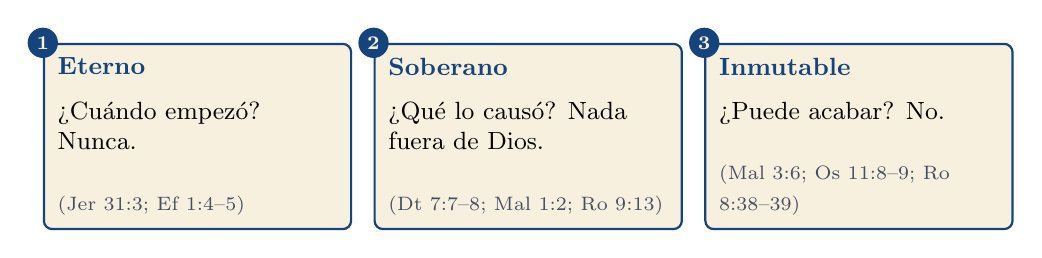
\begin{tikzpicture}
 \foreach \x/\n/\t/\d/\r in {0/1/{Eterno}/{¿Cuándo empezó? Nunca.}/{Jer 31:3; Ef 1:4--5},
   4.2/2/{Soberano}/{¿Qué lo causó? Nada fuera de Dios.}/{Dt 7:7--8; Mal 1:2; Ro 9:13},
   8.4/3/{Inmutable}/{¿Puede acabar? No.}/{Mal 3:6; Os 11:8--9; Ro 8:38--39}}{
  \node[caja,anchor=north] (b\n) at (\x,0) {\parbox[t][2.0cm][t]{3.55cm}{\RaggedRight
    {\small\textbf{\textcolor{azul}{\t}}}\\[5pt]\small \d\par\vfill{\scriptsize\color{gris}(\r)}}};
  \node[circle,fill=azul,text=papiro,font=\scriptsize\bfseries,inner sep=1.6pt] at (b\n.north west) {\n};}
\end{tikzpicture}\par\medskip
\begin{cita}Mas alábese en esto el que se hubiere de alabar: en entenderme y conocerme, que yo soy \SENOR, que hago misericordia, juicio y justicia en la tierra; porque estas cosas quiero, dice \SENOR.\fuente{(Jer 9:24, RVR1960)}\end{cita}
\scriptsize Tres preguntas, una sola respuesta: el amor de Dios no tiene principio, ni causa fuera de Dios, ni fin. Por eso es también santo, y se muestra infinito y lleno de gracia en Cristo (Ef 3:19; Ro 8:32).
\end{frame}

\begin{frame}{Clasificación}
\begin{columns}[c,onlytextwidth]
\begin{column}{0.50\textwidth}
\begin{tcolorbox}[colback=papiro,colframe=dorado,boxrule=1.2pt,arc=3pt]
\small\textbf{\textcolor{azul}{Ser}} (¿qué es?): Preexistente, Uno, \destacar{Amor}, Espíritu.
\end{tcolorbox}
\small\begin{itemize}
\item \textbf{Incomunicable} en su plenitud: solo el amor de Dios es eterno, sin causa fuera de sí e invariable.
\item \textbf{Comunicable} como reflejo: ``si Dios nos ha amado así, debemos también nosotros amarnos unos a otros'' (1 Jn 4:11).
\end{itemize}
\end{column}
\begin{column}{0.46\textwidth}
\begin{cita}Nosotros le amamos a él, porque él nos amó primero.\fuente{(1 Jn 4:19, RVR1960)}\end{cita}
\small Ese ``primero'' (\grc{πρῶτος}) abre los tres rasgos: un amor que precede (eterno), sin causa en nosotros (soberano) y que no depende de nosotros para seguir (inmutable).\par\medskip
\precision{clasificación propuesta; queda sujeta a tu revisión.}
\end{column}
\end{columns}
\end{frame}

% ------------------------------------------------------------------
\section{1 Juan 4}

\begin{frame}{El contexto de 1 Juan}
\small\begin{itemize}
\item Iglesias sacudidas por maestros que se fueron de la comunidad y negaban que Jesús fuera el Cristo venido en carne (1 Jn 2:18--19, 22; 4:1--3).
\item Tres pruebas de la vida verdadera: \destacar{creer} que Jesús es el Hijo, \destacar{obedecer} sus mandamientos, \destacar{amar} a los hermanos.
\item En el capítulo 4, la tercera prueba se apoya en la teología más alta de la carta: el amor entre hermanos viene de lo que Dios \emph{es}.
\end{itemize}\medskip
\precision{1 Juan no es de Pablo. Se usa como texto ancla porque contiene ``Dios es amor'' y porque así lo elegiste; la lectura paulina está en la sección ``En Cristo, con Pablo''.}
\end{frame}

\begin{frame}{Texto ancla: 1 Jn 4:7--10}
\fotolado{panel_1juan4.jpg}{Elaboración propia: 1 Jn 4:8 en uncial griega (NA28), con \emph{nomina sacra} \grc{ΘΝ} y \grc{ΘΣ}.}
\begin{columns}[c,onlytextwidth]
\begin{column}{0.58\textwidth}
\begin{cita}Amados, amémonos unos a otros; porque el amor es de Dios. Todo aquel que ama, es nacido de Dios, y conoce a Dios. El que no ama, no ha conocido a Dios; porque Dios es amor. En esto se mostró el amor de Dios para con nosotros, en que Dios envió a su Hijo unigénito al mundo, para que vivamos por él. En esto consiste el amor: no en que nosotros hayamos amado a Dios, sino en que él nos amó a nosotros, y envió a su Hijo en propiciación por nuestros pecados.\fuente{(1 Jn 4:7--10, RVR1960)}\end{cita}
\end{column}
\begin{column}{0.40\textwidth}\end{column}
\end{columns}
\end{frame}

\begin{frame}{1 Jn 4:11--16}
\begin{cita}Amados, si Dios nos ha amado así, debemos también nosotros amarnos unos a otros. Nadie ha visto jamás a Dios. Si nos amamos unos a otros, Dios permanece en nosotros, y su amor se ha perfeccionado en nosotros. En esto conocemos que permanecemos en él, y él en nosotros, en que nos ha dado de su Espíritu. Y nosotros hemos visto y testificamos que el Padre ha enviado al Hijo, el Salvador del mundo. Todo aquel que confiese que Jesús es el Hijo de Dios, Dios permanece en él, y él en Dios. Y nosotros hemos conocido y creído el amor que Dios tiene para con nosotros. Dios es amor; y el que permanece en amor, permanece en Dios, y Dios en él.\fuente{(1 Jn 4:11--16, RVR1960)}\end{cita}
\scriptsize El Padre envía y el Hijo es enviado como propiciación: el amor que Dios es se revela en el Padre que da a su Hijo (Jn 3:16).
\end{frame}

\begin{frame}{Filología: 1 Jn 4:8--10}
\renewcommand{\arraystretch}{1.15}\scriptsize
\begin{tabular}{@{}>{\RaggedRight\arraybackslash}p{3.0cm}>{\RaggedRight\arraybackslash}p{1.4cm}>{\RaggedRight\arraybackslash}p{7.6cm}@{}}
\toprule
\textbf{Término} & \textbf{Raíz} & \textbf{Sentido} \\ \midrule
\grc{ὁ θεὸς ἀγάπη ἐστίν} & \grc{ἀγάπη} & ``Dios es amor'': \emph{ho theós} lleva artículo (sujeto); \emph{agápē} no (predicado). No es reversible: no dice ``el amor es Dios''. \\
\grc{ἐν τούτῳ ἐφανερώθη} & \grc{φανερόω} & ``en esto se mostró'': se hizo visible en la historia, en el envío del Hijo. \\
\grc{τὸν μονογενῆ} & \grc{μόνος} & ``unigénito'', único en su clase (cf. Gn 22:2). \\
\grc{ἠγάπησεν ἡμᾶς} & \grc{ἀγαπάω} & ``él nos amó'': aoristo, un acto concreto; frente al perfecto \grc{ἠγαπήκαμεν}, ``nosotros hayamos amado''. \\
\grc{ἱλασμόν} & \grc{ἱλάσκομαι} & ``propiciación'': el sacrificio que aparta la ira. El amor no ignora el pecado: lo cubre a su propio costo. \\
\bottomrule
\end{tabular}
\end{frame}

\begin{frame}{Cuatro veces ``en esto''}
\small\renewcommand{\arraystretch}{1.25}
\begin{tabular}{@{}>{\RaggedRight\arraybackslash}p{1.2cm}>{\RaggedRight\arraybackslash}p{4.0cm}>{\RaggedRight\arraybackslash}p{6.8cm}@{}}
\toprule
\textbf{Verso} & \textbf{\grc{ἐν τούτῳ}\ldots} & \textbf{Respuesta} \\ \midrule
4:9 & se \destacar{mostró} el amor & Dios envió a su Hijo unigénito para que vivamos por él. \\
4:10 & \destacar{consiste} el amor & No en nuestro amor a Dios, sino en que él nos amó y envió a su Hijo en propiciación. \\
4:13 & \destacar{conocemos} que permanecemos & Nos ha dado de su Espíritu. \\
4:17 & se ha \destacar{perfeccionado} el amor & Tenemos confianza en el día del juicio. \\
\bottomrule
\end{tabular}\par\medskip
\scriptsize Primero lo que Dios es; luego cómo lo mostró (el envío), en qué consiste (la propiciación), cómo llega a nosotros (el Espíritu) y adónde nos lleva (confianza ante el juicio).
\end{frame}

% ------------------------------------------------------------------
\section{La palabra}

\begin{frame}{La raíz \emph{ahav}}
\begin{columns}[t,onlytextwidth]
\begin{column}{0.50\textwidth}\small
\heb{אָהַב} \emph{ahav}, ``amar''; \heb{אַהֲבָה} \emph{ahavá}, ``amor''. Unas 250 apariciones (Vine, 1999); conteo propio en BHS: 248 formas en 227 versículos.
\begin{itemize}
\item esposo y esposa (Gn 24:67; 29:20)
\item padre e hijo (Gn 22:2; 37:3)
\item amigos (1 S 18:1)
\item siervo y señor (Éx 21:5)
\item lealtad política (1 R 5:1 [5:15])
\end{itemize}
\scriptsize Es la palabra común del amor humano. Por eso sorprende que Dios la use de sí mismo.
\end{column}
\begin{column}{0.47\textwidth}
\begin{cita}Así sirvió Jacob por Raquel siete años; y le parecieron como pocos días, porque la amaba.\fuente{(Gn 29:20, RVR1960)}\end{cita}
\begin{cita}\ldots{} el alma de Jonatán quedó ligada con la de David, y lo amó Jonatán como a sí mismo.\fuente{(1 S 18:1, RVR1960)}\end{cita}
\scriptsize\heb{נִקְשְׁרָה} \emph{niqsherá}, ``quedó ligada'', atada como con un nudo.
\end{column}
\end{columns}
\end{frame}

\begin{frame}{La primera vez: el hijo amado}
\begin{center}\heb{קַח־נָא אֶת־בִּנְךָ אֶת־יְחִידְךָ אֲשֶׁר־אָהַבְתָּ אֶת־יִצְחָק}\end{center}
\begin{cita}Y dijo: Toma ahora tu hijo, tu único, Isaac, a quien amas, y vete a tierra de Moriah, y ofrécelo allí en holocausto sobre uno de los montes que yo te diré.\fuente{(Gn 22:2, RVR1960)}\end{cita}
\begin{columns}[t,onlytextwidth]
\begin{column}{0.50\textwidth}\scriptsize
\begin{itemize}
\item \heb{יְחִידְךָ} \emph{yejidjá}: ``tu único''.
\item \heb{אֲשֶׁר־אָהַבְתָּ}: primera vez que aparece ``amar'' en la Biblia.
\item LXX: \grc{τὸν ἀγαπητόν, ὃν ἠγάπησας}, ``al amado, al que amaste''.
\end{itemize}
\end{column}
\begin{column}{0.47\textwidth}\scriptsize
\begin{itemize}
\item ``Este es mi Hijo amado'' (\grc{ὁ ἀγαπητός}, Mt 3:17).
\item ``El que no escatimó ni a su propio Hijo'' (Ro 8:32) $\leftrightarrow$ \grc{οὐκ ἐφείσω τοῦ υἱοῦ σου τοῦ ἀγαπητοῦ} (Gn 22:16 LXX).
\end{itemize}
\precision{eco verbal (\grc{φείδομαι}), lectura tipológica (Moo, 1996; Dunn, 1998).}
\end{column}
\end{columns}
\end{frame}

\begin{frame}{El amor del pacto: el Shemá}
\begin{center}\heb{שְׁמַע יִשְׂרָאֵל יְהוָה אֱלֹהֵינוּ יְהוָה אֶחָד}\\[1pt]\heb{וְאָהַבְתָּ אֵת יְהוָה אֱלֹהֶיךָ בְּכָל־לְבָבְךָ וּבְכָל־נַפְשְׁךָ וּבְכָל־מְאֹדֶךָ}\end{center}
\begin{cita}Oye, Israel: \SENOR{} nuestro Dios, \SENOR{} uno es. Y amarás a \SENOR{} tu Dios de todo tu corazón, y de toda tu alma, y con todas tus fuerzas.\fuente{(Dt 6:4--5, RVR1960)}\end{cita}
\renewcommand{\arraystretch}{1.05}\scriptsize
\begin{tabular}{@{}>{\RaggedRight\arraybackslash}p{2.3cm}>{\RaggedRight\arraybackslash}p{9.6cm}@{}}
\heb{וְאָהַבְתָּ} & ``y amarás'': mandato. El amor se puede mandar porque es lealtad del corazón, no solo emoción. \\
\heb{לְבָבְךָ} & ``tu corazón'': centro de la voluntad y el pensamiento. \\
\heb{מְאֹדֶךָ} & ``tus fuerzas'': literalmente ``tu mucho'', todo lo que uno tiene y puede. \\
\end{tabular}\par\smallskip
\precision{``amar'' y ``guardar los mandamientos'' tienen paralelos en los tratados del antiguo Oriente (Moran, 1963); Deuteronomio funda el amor de Israel en el amor previo y gratuito de Dios (Dt 7:7--8; 10:15).}
\end{frame}

\begin{frame}{El espectro: ``amor'' en la RVR1960}
\scriptsize\renewcommand{\arraystretch}{1.05}
\begin{tabular}{@{}>{\RaggedRight\arraybackslash}p{3.3cm}>{\RaggedRight\arraybackslash}p{3.4cm}>{\RaggedRight\arraybackslash}p{5.3cm}@{}}
\toprule
\textbf{Término} & \textbf{Sentido base} & \textbf{Textos y frecuencia} \\ \midrule
\heb{אָהַב}, \heb{אַהֲבָה} \emph{ahav, ahavá} & amar, amor & $\approx$\,250; la palabra principal \\
\heb{דּוֹד} \emph{dod} & amado; amores & sobre todo Cantares; Is 5:1; Ez 16:8 \\
\heb{יָדִיד} \emph{yedid} & amado, querido & Dt 33:12; Sal 127:2; Jer 11:15 \\
\heb{חָשַׁק} \emph{jashaq} & ligarse por amor & Dt 7:7; 10:15; Sal 91:14 \\
\heb{רָחַם} \emph{rajam} & amar entrañablemente & Sal 18:1 [18:2]; arameo: ``amar'' \\
\heb{לְמַעַן}, \heb{בַּעֲבוּר} & ``a causa de'' & ``por amor de'' (73 veces): no es vocabulario de amor \\ \midrule
\grc{ἀγαπάω}; \grc{ἀγάπη}; \grc{ἀγαπητός} & amar; amor; amado & 143; 116; 61 (NA27) \\
\grc{φιλέω}; \grc{φίλος} & querer; amigo & 25; 29 \\
\grc{φιλαδελφία}, \grc{φιλανθρωπία} & amor fraternal; a los hombres & Ro 12:10; Tit 3:4 \\
\grc{σπλάγχνα} & entrañas, afecto & ``entrañable amor'' (Flp 1:8) \\
\bottomrule
\end{tabular}\par\smallskip
\precision{conteo propio (RVR1960 sin títulos, BHS y NA27 con Strong): ``amor, amar, amado, amante'' = \textbf{713 veces en 608 versículos} (346 AT, 367 NT); verificar en e-Sword.}
\end{frame}

\begin{frame}{Dos palabras más: \emph{jashaq} y \emph{rjm}}
\begin{columns}[t,onlytextwidth]
\begin{column}{0.49\textwidth}
\begin{tcolorbox}[colback=papiro,colframe=azul,boxrule=0.8pt,arc=3pt,title={\heb{חָשַׁק} \emph{jashaq}},coltitle=papiro,colbacktitle=azul,fonttitle=\small\bfseries]
\small Sentido concreto: ``ligar, sujetar'' (las molduras que ciñen las columnas, Éx 27:17; 38:17). De afecto: poner el corazón sobre alguien y quedar ligado (Gn 34:8; Dt 7:7; 10:15).
\end{tcolorbox}
\end{column}
\begin{column}{0.49\textwidth}
\begin{tcolorbox}[colback=papiro,colframe=azul,boxrule=0.8pt,arc=3pt,title={\heb{רחם} \emph{rjm}},coltitle=papiro,colbacktitle=azul,fonttitle=\small\bfseries]
\small Ónkelos traduce ``amarás'' (Dt 6:5) con \heb{וְתִרְחַם}. En arameo es el verbo común de ``amar''; en hebreo da \emph{rajamím}, las entrañas de misericordia.
\end{tcolorbox}
\end{column}
\end{columns}\medskip
\small El amor y la misericordia de Dios comparten raíz (véase el capítulo sobre la misericordia).
\end{frame}

\begin{frame}{\emph{Agapē} y \emph{phileō}}
\begin{columns}[c,onlytextwidth]
\begin{column}{0.52\textwidth}\small
\begin{itemize}
\item La LXX traduce \emph{ahav} casi siempre con \grc{ἀγαπάω} (172 de 227 versículos; \grc{φιλέω} en 23).
\item \grc{ἀγάπη} era rara antes de la LXX (Cantares); el NT la vuelve la palabra central.
\item \grc{ἔρως} nunca aparece en el NT.
\end{itemize}
\end{column}
\begin{column}{0.45\textwidth}
\begin{tcolorbox}[colback=dorado!10,colframe=dorado!85!azul,boxrule=0.6pt,arc=2pt,title={Falacia de la raíz},fonttitle=\scriptsize\bfseries,coltitle=azuloscuro,colbacktitle=dorado!30]
\scriptsize \emph{Agapē} no significa por sí sola ``amor divino''. Amnón ``amó'' a Tamar con \grc{ἀγαπάω} (2 S 13:15 LXX); Demas ``amando'' este mundo (2 Ti 4:10); el Padre ama al Hijo con \grc{ἀγαπάω} (Jn 3:35) y con \grc{φιλέω} (Jn 5:20) (Carson, 2013).
\end{tcolorbox}
\end{column}
\end{columns}\medskip
\small Lo que da contenido a \emph{agapē} no es la palabra, sino el acto: ``En esto consiste el amor\ldots{} envió a su Hijo'' (1 Jn 4:10).
\end{frame}

\begin{frame}{De \emph{ahavá} a \emph{agapē}}
\centering
\begin{tikzpicture}[font=\small, node distance=0.8cm]
 \tikzset{b/.style={caja,font=\small,text width=3.4cm,align=center}}
 \node[b] (h) {\textbf{Hebreo}\\ \heb{וְאַהֲבַת עוֹלָם אֲהַבְתִּיךְ}\\ {\footnotesize Jer 31:3}};
 \node[b,right=of h] (l) {\textbf{LXX}\\ \grc{ἀγάπησιν αἰωνίαν ἠγάπησά σε}\\ {\footnotesize Jer 38:3}};
 \node[b,right=of l] (p) {\textbf{Pablo}\\ \grc{ὁ ἀγαπήσας ἡμᾶς καὶ δοὺς παράκλησιν αἰωνίαν}\\ {\footnotesize 2 Ts 2:16}};
 \draw[-{Latex[length=3mm]},dorado,line width=1.4pt] (h)--(l);
 \draw[-{Latex[length=3mm]},dorado,line width=1.4pt] (l)--(p);
\end{tikzpicture}\par\bigskip
\small El amor eterno pasa del profeta al apóstol: Dios ``nos amó y nos dio consolación eterna'' (2 Ts 2:16).\par\medskip
{\fontsize{5}{6}\selectfont\color{gris}\textit{Nota.} Elaboración propia (BHS, Rahlfs-Hanhart, NA28).}
\end{frame}

% ------------------------------------------------------------------
\section{El Nombre}

\begin{frame}{Jedidías: ``amado del \SENOR''}
\begin{center}\heb{וַיִּקְרָא אֶת־שְׁמוֹ שְׁלֹמֹה וַיהוָה אֲהֵבוֹ}\\[1pt]\heb{וַיִּקְרָא אֶת־שְׁמוֹ יְדִידְיָהּ בַּעֲבוּר יְהוָה}\end{center}
\begin{cita}\ldots{} y llamó su nombre Salomón, al cual amó \SENOR, y envió un mensaje por medio de Natán profeta; así llamó su nombre Jedidías, a causa de \SENOR.\fuente{(2 S 12:24--25, RVR1960)}\end{cita}
\begin{columns}[t,onlytextwidth]
\begin{column}{0.50\textwidth}\scriptsize
\begin{itemize}
\item \heb{יְדִידְיָהּ}: \emph{yedid}, ``amado'', + \emph{Yah}. Único lugar.
\item \heb{בַּעֲבוּר יְהוָה}: ``a causa del \SENOR'', no de David ni del niño.
\end{itemize}
\end{column}
\begin{column}{0.47\textwidth}\scriptsize
El nombre llega por Natán, el profeta que denunció el pecado (12:7): el amor soberano se nombra donde menos se esperaba.\par
\precision{lectura propia (2 S 12:13--25). La Torá no tiene un nombre de Dios formado con \emph{ahav}; Dios es llamado según sus obras (\emph{Shemot Rabá} 3:6).}
\end{column}
\end{columns}
\end{frame}

\begin{frame}{``El Dios de amor y de paz''}
\begin{cita}Por lo demás, hermanos, tened gozo, perfeccionaos, consolaos, sed de un mismo sentir, y vivid en paz; y el Dios de paz y de amor estará con vosotros.\fuente{(2 Co 13:11, RVR1960)}\end{cita}
\renewcommand{\arraystretch}{1.12}\scriptsize
\begin{tabular}{@{}>{\RaggedRight\arraybackslash}p{3.6cm}>{\RaggedRight\arraybackslash}p{8.3cm}@{}}
\grc{ὁ θεὸς τῆς ἀγάπης καὶ εἰρήνης} & ``el Dios del amor y de la paz'': el griego pone primero el amor. Única vez en el NT (conteo propio, NA27). \\
\grc{ἔσται μεθ᾽ ὑμῶν} & ``estará con vosotros'': como \heb{אֶהְיֶה עִמָּךְ}, ``yo estaré contigo'' (Éx 3:12). \\
\end{tabular}\par\medskip
\begin{cita}La gracia del Señor Jesucristo, el amor de Dios, y la comunión del Espíritu Santo sean con todos vosotros. Amén.\fuente{(2 Co 13:14, RVR1960)}\end{cita}
\end{frame}

\begin{frame}{Nombres y títulos que revelan el amor}
\scriptsize\renewcommand{\arraystretch}{1.15}
\begin{tabular}{@{}>{\RaggedRight\arraybackslash}p{2.8cm}>{\RaggedRight\arraybackslash}p{3.3cm}>{\RaggedRight\arraybackslash}p{1.8cm}>{\RaggedRight\arraybackslash}p{4.0cm}@{}}
\toprule
\textbf{Nombre o título} & \textbf{Hebreo / griego} & \textbf{Texto} & \textbf{Qué revela} \\ \midrule
Jedidías & \heb{יְדִידְיָהּ} & 2 S 12:25 & Amor soberano nombrado después del pecado. \\
``Dios es amor'' & \grc{ὁ θεὸς ἀγάπη ἐστίν} & 1 Jn 4:8, 16 & El amor como lo que Dios es. \\
Dios del amor y de la paz & \grc{ὁ θεὸς τῆς ἀγάπης} & 2 Co 13:11 & El amor en el nombre de Dios. \\
El Amado & \grc{ὁ ἠγαπημένος} & Ef 1:6 & El Hijo en quien somos aceptados. \\
El Hijo de su amor & \grc{ὁ υἱὸς τῆς ἀγάπης αὐτοῦ} & Col 1:13 & El amor eterno del Padre por el Hijo. \\
``El que ama a su pueblo Israel'' & \heb{אוֹהֵב עַמּוֹ יִשְׂרָאֵל} & Liturgia & El amor de pacto, confesado en la oración. \\
\bottomrule
\end{tabular}\par\smallskip
\precision{la última fórmula cierra la bendición \emph{Ahavat olam} (sidur asquenazí); la de la mañana, \emph{Ahavá rabbá}, cierra con \heb{הַבּוֹחֵר בְּעַמּוֹ יִשְׂרָאֵל בְּאַהֲבָה}, ``que escoges a tu pueblo Israel con amor''. Son litúrgicas, no bíblicas.}
\end{frame}

% ------------------------------------------------------------------
\section{Definición}

\begin{frame}{¿Qué es el amor de Dios?}
\begin{tcolorbox}[colback=papiro,colframe=azul,boxrule=1pt,arc=3pt]
\small El amor de Dios es la perfección eterna de su ser por la cual Dios, en la comunión del Padre y del Hijo, se da a sí mismo y quiere y procura el bien de aquellos a quienes ama. Es \destacar{eterno}, porque no tuvo principio (Jer 31:3; Jn 17:24; Ef 1:4); \destacar{soberano}, porque su única causa está en Dios mismo (Dt 7:7--8; Ef 1:5); e \destacar{inmutable}, porque nada en la criatura lo puede apagar (Mal 3:6; Ro 8:38--39). Es santo y no sentimental (1 Jn 1:5; He 12:6), y se mostró de una vez para siempre en el envío del Hijo como propiciación (1 Jn 4:9--10; Ro 5:8).
\end{tcolorbox}
\precision{síntesis propuesta en esta serie a partir de los textos y de Pink (2020, cap.~16); queda sujeta a tu revisión.}
\end{frame}

\begin{frame}{Amor antes de la creación}
\begin{columns}[c,onlytextwidth]
\begin{column}{0.50\textwidth}
\begin{cita}Padre, aquellos que me has dado, quiero que donde yo estoy, también ellos estén conmigo, para que vean mi gloria que me has dado; porque me has amado desde antes de la fundación del mundo.\fuente{(Jn 17:24, RVR1960)}\end{cita}
\end{column}
\begin{column}{0.47\textwidth}\small
Si Dios \emph{es} amor, su amor no depende de que exista una criatura.
\begin{itemize}
\item El Padre ama al Hijo (Jn 3:35; 5:20; 15:9).
\item Ese amor llega a nosotros: ``el amor de Dios ha sido derramado en nuestros corazones'' (Ro 5:5).
\end{itemize}
\precision{el amor del Padre al Hijo antes de crear (Jn 17:24; 3:35) es lectura cristiana, no la letra de 1 Juan.}
\end{column}
\end{columns}
\end{frame}

\begin{frame}{Distinciones necesarias}
\small\renewcommand{\arraystretch}{1.18}
\begin{tabular}{@{}>{\RaggedRight\arraybackslash}p{5.4cm}>{\RaggedRight\arraybackslash}p{6.4cm}@{}}
\toprule
\textbf{El amor de Dios\ldots} & \textbf{Textos} \\ \midrule
del Padre por el Hijo & Jn 3:35; 5:20; 17:24 \\
providencial, por toda su creación & Mt 5:45; Sal 145:9 \\
salvador, hacia el mundo caído & Jn 3:16 \\
electivo, por su pueblo & Dt 7:7--8; Ef 5:25 \\
dentro del pacto, ligado a la obediencia & Jn 15:10; Jud 21 \\
\bottomrule
\end{tabular}\par\smallskip
\scriptsize Carson (2000). Confundirlos lleva a un amor tan general que no salva a nadie, o tan particular que Dios no tendría bondad hacia el mundo.\par
\precision{Pink (2020, p.~88) lee el ``mundo'' de Jn 3:16 en contraste con los judíos y reserva ``amor'' para los elegidos; Carson (2000) sostiene la elección y una verdadera disposición amorosa hacia el mundo. Se señala sin resolver.}
\end{frame}

% ------------------------------------------------------------------
\section{Teología}

\begin{frame}{Eterno: Jer 31:3}
\fotolado{panel_jeremias31.jpg}{Elaboración propia: Jer 31:3 en texto hebreo consonántico (BHS).}
\begin{columns}[c,onlytextwidth]
\begin{column}{0.58\textwidth}
\begin{cita}\SENOR{} se manifestó a mí hace ya mucho tiempo, diciendo: Con amor eterno te he amado; por tanto, te prolongué mi misericordia.\fuente{(Jer 31:3, RVR1960)}\end{cita}
\scriptsize\renewcommand{\arraystretch}{1.08}
\begin{tabular}{@{}>{\RaggedRight\arraybackslash}p{2.2cm}>{\RaggedRight\arraybackslash}p{5.3cm}@{}}
\heb{אַהֲבַת עוֹלָם} & ``amor de siglo'': tiempo sin límite visible, hacia atrás y hacia adelante. \\
\heb{אֲהַבְתִּיךְ} & ``te he amado'': perfecto; sufijo femenino, la ``virgen de Israel'' (31:4). \\
\heb{מְשַׁכְתִּיךְ חָסֶד} & ``te atraje con \emph{jésed}''; \emph{mashaj}, ``tirar, prolongar''. LXX \grc{εἵλκυσά σε}. \\
\end{tabular}\par\smallskip
\precision{el Libro de la Consolación (Jer 30--33) habla a un pueblo en el exilio. \heb{מֵרָחוֹק}: ``desde lejos'' o ``hace mucho tiempo''.}
\end{column}
\begin{column}{0.40\textwidth}\end{column}
\end{columns}
\end{frame}

\begin{frame}{Eterno: ``antes de la fundación del mundo''}
\begin{cita}Según nos escogió en él antes de la fundación del mundo, para que fuésemos santos y sin mancha delante de él, en amor habiéndonos predestinado para ser adoptados hijos suyos por medio de Jesucristo, según el puro afecto de su voluntad.\fuente{(Ef 1:4--5, RVR1960)}\end{cita}
\small\begin{itemize}
\item El amor que eligió \grc{πρὸ καταβολῆς κόσμου} es el mismo con que el Padre amó al Hijo ``desde antes de la fundación del mundo'' (Jn 17:24).
\item ``Con cuerdas de amor'' los atraje (\heb{אֶמְשְׁכֵם}, Os 11:4); ``si el Padre\ldots{} no le trajere'' (\grc{ἑλκύσῃ}, Jn 6:44).
\end{itemize}
\begin{cita}Qué tranquilizador es para el corazón que, como el amor de Dios hacia mí no tuvo principio, ¡no puede tener final!\fuente{(Pink, 2020, p.~85)}\end{cita}
\precision{Jer 38:3 LXX $\leftrightarrow$ Jn 6:44 es un posible eco verbal, lectura propia.}
\end{frame}

\begin{frame}{Soberano: Dt 7:6--8}
\begin{center}\heb{לֹא מֵרֻבְּכֶם מִכָּל־הָעַמִּים חָשַׁק יְהוָה בָּכֶם וַיִּבְחַר בָּכֶם}\\[1pt]\heb{כִּי־אַתֶּם הַמְעַט מִכָּל־הָעַמִּים כִּי מֵאַהֲבַת יְהוָה אֶתְכֶם}\end{center}
\begin{cita}\ldots{} No por ser vosotros más que todos los pueblos os ha querido \SENOR{} y os ha escogido, pues vosotros erais el más insignificante de todos los pueblos; sino por cuanto \SENOR{} os amó, y quiso guardar el juramento que juró a vuestros padres, os ha sacado \SENOR{} con mano poderosa\ldots\fuente{(Dt 7:7--8, RVR1960)}\end{cita}
\renewcommand{\arraystretch}{1.05}\scriptsize
\begin{tabular}{@{}>{\RaggedRight\arraybackslash}p{2.6cm}>{\RaggedRight\arraybackslash}p{9.3cm}@{}}
\heb{חָשַׁק בָּכֶם} & ``se ligó a vosotros'' (RVR: ``os ha querido''). \\
\heb{וַיִּבְחַר} & ``y escogió'': el amor precede a la elección y la explica. \\
\heb{מֵאַהֲבַת יְהוָה} & ``por el amar del \SENOR'': la única causa nombrada. \\
\end{tabular}\par\smallskip
\small Dios no los amó porque fueran muchos ni buenos (Dt 9:4--6): los amó porque los amó.
\end{frame}

\begin{frame}{Soberano: el dueño del universo se ligó a unos nómadas}
\begin{cita}He aquí, de \SENOR{} tu Dios son los cielos, y los cielos de los cielos, la tierra, y todas las cosas que hay en ella. Solamente de tus padres se agradó \SENOR{} para amarlos, y escogió su descendencia después de ellos, a vosotros, de entre todos los pueblos, como en este día.\fuente{(Dt 10:14--15, RVR1960)}\end{cita}
\begin{cita}Yo sanaré su rebelión, los amaré de pura gracia; porque mi ira se apartó de ellos.\fuente{(Os 14:4 [14:5], RVR1960)}\end{cita}
\small\heb{נְדָבָה} \emph{nedavá}, ``de pura gracia'': la palabra de las ofrendas voluntarias (Éx 35:29; Lv 7:16). El amor de Dios es una ofrenda que nadie le exige.\par\smallskip
\scriptsize Pablo: ``según el puro afecto (\grc{εὐδοκία}) de su voluntad'' (Ef 1:5). Soberano no es arbitrario: sus razones están en Dios, en su juramento y en su Hijo.
\end{frame}

\begin{frame}{Soberano: ``A Jacob amé''}
\begin{columns}[t,onlytextwidth]
\begin{column}{0.50\textwidth}
\begin{center}\heb{אָהַבְתִּי אֶתְכֶם אָמַר יְהוָה}\end{center}
\begin{cita}Yo os he amado, dice \SENOR; y dijisteis: ¿En qué nos amaste? ¿No era Esaú hermano de Jacob? dice \SENOR. Y amé a Jacob, y a Esaú aborrecí\ldots\fuente{(Mal 1:2--3, RVR1960)}\end{cita}
\end{column}
\begin{column}{0.47\textwidth}
\begin{cita}(pues no habían aún nacido, ni habían hecho aún ni bien ni mal, para que el propósito de Dios conforme a la elección permaneciese, no por las obras sino por el que llama), se le dijo: El mayor servirá al menor. Como está escrito: A Jacob amé, mas a Esaú aborrecí.\fuente{(Ro 9:11--13, RVR1960)}\end{cita}
\end{column}
\end{columns}
\precision{``amar/aborrecer'' es lenguaje de elección: Jacob amó a Raquel ``más que a Lea'', la ``menospreciada'' (\heb{שְׂנוּאָה}, Gn 29:30--31); ``aborrecer'' padre y madre (Lc 14:26) = ``amar más'' (Mt 10:37). Se discute si Pablo habla de pueblos o de personas (Moo, 1996; Dunn, 1998).}
\end{frame}

\begin{frame}{Inmutable: Mal 3:6}
\begin{center}\heb{כִּי אֲנִי יְהוָה לֹא שָׁנִיתִי וְאַתֶּם בְּנֵי־יַעֲקֹב לֹא כְלִיתֶם}\end{center}
\begin{cita}Porque yo \SENOR{} no cambio; por esto, hijos de Jacob, no habéis sido consumidos.\fuente{(Mal 3:6, RVR1960)}\end{cita}
\renewcommand{\arraystretch}{1.08}\scriptsize
\begin{tabular}{@{}>{\RaggedRight\arraybackslash}p{2.6cm}>{\RaggedRight\arraybackslash}p{9.3cm}@{}}
\heb{לֹא שָׁנִיתִי} & ``no he cambiado''; LXX \grc{οὐκ ἠλλοίωμαι}, ``no he sido alterado''. \\
\heb{בְּנֵי־יַעֲקֹב} & ``hijos de Jacob'': el mismo Jacob de 1:2, ``Y amé a Jacob''. \\
\heb{לֹא כְלִיתֶם} & ``no habéis sido consumidos'', no habéis llegado a vuestro fin. \\
\end{tabular}\par\medskip
\begin{cita}Porque los montes se moverán, y los collados temblarán, pero no se apartará de ti mi misericordia, ni el pacto de mi paz se quebrantará, dijo \SENOR, el que tiene misericordia de ti.\fuente{(Is 54:10, RVR1960)}\end{cita}
\precision{unir Mal 1:2 y 3:6 por el nombre ``Jacob'' es lectura propia.}
\end{frame}

\begin{frame}{Inmutable: ``los amó hasta el fin''}
\begin{columns}[t,onlytextwidth]
\begin{column}{0.49\textwidth}
\begin{cita}Porque fuerte es como la muerte el amor; Duros como el Seol los celos\ldots{} Las muchas aguas no podrán apagar el amor, Ni lo ahogarán los ríos.\fuente{(Cnt 8:6--7, RVR1960)}\end{cita}
\end{column}
\begin{column}{0.48\textwidth}
\begin{cita}\ldots{} como había amado a los suyos que estaban en el mundo, los amó hasta el fin.\fuente{(Jn 13:1, RVR1960)}\end{cita}
\scriptsize\grc{εἰς τέλος ἠγάπησεν αὐτούς}: hasta el final y hasta el extremo, la noche en que lo negarían y huirían.
\end{column}
\end{columns}\medskip
\begin{tcolorbox}[colback=dorado!10,colframe=dorado!85!azul,boxrule=0.6pt,arc=2pt]
\small Dios cambia su trato (consuela, corrige, disciplina), no su disposición: ``el Señor al que ama, disciplina'' (He 12:6). Como observa Pink (2020, p.~90), Dios ``varía las dispensaciones de su Providencia'', pero no porque ``su afecto haya cambiado''.
\end{tcolorbox}
\end{frame}

\begin{frame}{Santo, no sentimental}
\begin{columns}[c,onlytextwidth]
\begin{column}{0.50\textwidth}\small
El amor eterno, soberano e inmutable no es indulgencia. Juan escribe ``Dios es luz'' (1 Jn 1:5) antes de ``Dios es amor'' (4:8), y define el amor por la propiciación (4:10). El Cantar pone en paralelo \heb{אַהֲבָה}, amor, y \heb{קִנְאָה}, celo (Cnt 8:6): el amor de Dios no tolera rivales. Por eso no deja intacto el pecado, sino que lo juzga en el Hijo para salvar al pecador, y la cruz revela a la vez la ira y el amor (Ro 3:25--26; 5:8--9).
\end{column}
\begin{column}{0.46\textwidth}
\begin{cita}El amor de Dios no está regulado por el capricho, la pasión o el sentimiento, sino por principios\ldots{} su amor nunca entra en conflicto con su santidad.\fuente{(Pink, 2020, p.~87)}\end{cita}
\end{column}
\end{columns}
\end{frame}

% ------------------------------------------------------------------
\section{Encuentro en Israel}

\begin{frame}{Oseas: un matrimonio como profecía}
\begin{columns}[t,onlytextwidth]
\begin{column}{0.46\textwidth}\small
\begin{itemize}
\item Reino del norte, siglo VIII a.\,e.\,c., antes de la caída de Samaria (722).
\item ``Ve, tómate una mujer fornicaria\ldots'' (Os 1:2).
\item Hijos con nombres de juicio: \emph{Lo-ruhamá}, ``no compadecida''; \emph{Lo-ammí}, ``no pueblo mío'' (1:6, 9).
\item Gomer lo abandona. Llega una segunda orden.
\end{itemize}
\end{column}
\begin{column}{0.51\textwidth}
\begin{center}\heb{לֵךְ אֱהַב־אִשָּׁה אֲהֻבַת רֵעַ וּמְנָאָפֶת}\\[1pt]\heb{כְּאַהֲבַת יְהוָה אֶת־בְּנֵי יִשְׂרָאֵל}\end{center}
\begin{cita}Me dijo otra vez \SENOR: Ve, ama a una mujer amada de su compañero, aunque adúltera, como el amor de \SENOR{} para con los hijos de Israel, los cuales miran a dioses ajenos, y aman tortas de pasas.\fuente{(Os 3:1, RVR1960)}\end{cita}
\end{column}
\end{columns}
\end{frame}

\begin{frame}{Os 3:1: cuatro veces \emph{ahav}}
\centering
\begin{tikzpicture}[font=\small,node distance=0.5cm]
 \node[caja,font=\small,text width=2.6cm,align=center] (a) {\heb{אֱהַב}\\ ``ama'' (orden de Dios)};
 \node[caja,font=\small,text width=2.6cm,align=center,right=of a] (b) {\heb{אֲהֻבַת רֵעַ}\\ ``amada de otro''};
 \node[draw=dorado,line width=1.6pt,fill=azul,text=papiro,rounded corners=3pt,text width=2.6cm,align=center,inner sep=5pt,right=of b] (c) {\heb{כְּאַהֲבַת יְהוָה}\\ ``como el amor del \SENOR''};
 \node[caja,font=\small,text width=2.6cm,align=center,right=of c] (d) {\heb{וְאֹהֲבֵי}\\ ``aman tortas de pasas''};
\end{tikzpicture}\par\bigskip
\small\begin{itemize}
\item Dos amores frente a frente: el de Dios, fiel; el de su pueblo, dividido.
\item Oseas compró a su esposa (3:2) y le dio tiempo para volver (3:3--5).
\item \heb{אֲשִׁישֵׁי עֲנָבִים}, ``tortas de pasas'': probablemente ofrendas de los cultos de fertilidad.
\end{itemize}
\end{frame}

\begin{frame}{``Cuando Israel era muchacho, yo lo amé''}
\begin{center}\heb{כִּי נַעַר יִשְׂרָאֵל וָאֹהֲבֵהוּ וּמִמִּצְרַיִם קָרָאתִי לִבְנִי}\end{center}
\begin{cita}Cuando Israel era muchacho, yo lo amé, y de Egipto llamé a mi hijo. Cuanto más yo los llamaba, tanto más se alejaban de mí; a los baales sacrificaban, y a los ídolos ofrecían sahumerios. Yo con todo eso enseñaba a andar al mismo Efraín, tomándole de los brazos; y no conoció que yo le cuidaba. Con cuerdas humanas los atraje, con cuerdas de amor\ldots\fuente{(Os 11:1--4, RVR1960)}\end{cita}
\small El amor eterno en lenguaje doméstico: un padre que enseña a caminar a un niño. Empezó antes de cualquier respuesta y es la causa del éxodo (cf. Dt 7:8). Mateo verá aquí a Jesús, el Hijo que recorre el camino de Israel (Mt 2:15).
\end{frame}

\begin{frame}{``¿Cómo podré abandonarte, oh Efraín?''}
\fotolado{panel_oseas11.jpg}{Elaboración propia: Os 11:8 en texto hebreo consonántico (BHS).}
\begin{columns}[c,onlytextwidth]
\begin{column}{0.58\textwidth}
\begin{cita}¿Cómo podré abandonarte, oh Efraín? ¿Te entregaré yo, Israel? ¿Cómo podré yo hacerte como Adma, o ponerte como a Zeboim? Mi corazón se conmueve dentro de mí, se inflama toda mi compasión. No ejecutaré el ardor de mi ira, ni volveré para destruir a Efraín; porque Dios soy, y no hombre, el Santo en medio de ti; y no entraré en la ciudad.\fuente{(Os 11:8--9, RVR1960)}\end{cita}
\scriptsize\heb{נֶהְפַּךְ עָלַי לִבִּי}, ``se me da vuelta el corazón'': \emph{hafaj} es el verbo de la destrucción de Sodoma (Gn 19:25; Dt 29:23). En lugar de trastornar a Efraín, Dios trastorna su propio corazón.\par
\precision{juego de palabras como lectura propia; Adma y Zeboim cayeron con Sodoma.}
\end{column}
\begin{column}{0.40\textwidth}\end{column}
\end{columns}
\end{frame}

\begin{frame}{Oseas: los tres rasgos juntos}
\centering
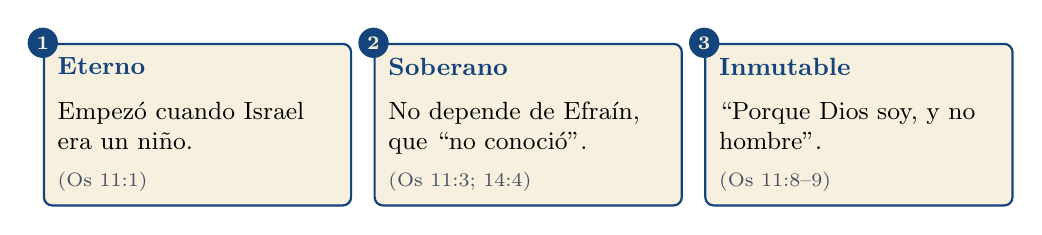
\begin{tikzpicture}
 \foreach \x/\n/\t/\d/\r in {0/1/{Eterno}/{Empezó cuando Israel era un niño.}/{Os 11:1},
   4.2/2/{Soberano}/{No depende de Efraín, que ``no conoció''.}/{Os 11:3; 14:4},
   8.4/3/{Inmutable}/{``Porque Dios soy, y no hombre''.}/{Os 11:8--9}}{
  \node[caja,anchor=north] (b\n) at (\x,0) {\parbox[t][1.7cm][t]{3.55cm}{\RaggedRight
    {\small\textbf{\textcolor{azul}{\t}}}\\[5pt]\small \d\par\vfill{\scriptsize\color{gris}(\r)}}};
  \node[circle,fill=azul,text=papiro,font=\scriptsize\bfseries,inner sep=1.6pt] at (b\n.north west) {\n};}
\end{tikzpicture}\par\bigskip
\begin{cita}Como también en Oseas dice: Llamaré pueblo mío al que no era mi pueblo, Y a la no amada, amada.\fuente{(Ro 9:25, RVR1960; cf. Os 2:23)}\end{cita}
\end{frame}

% ------------------------------------------------------------------
\section{En el judaísmo}

\begin{frame}{El amor antes del Shemá}
\begin{columns}[c,onlytextwidth]
\begin{column}{0.52\textwidth}\small
\begin{itemize}
\item Antes del Shemá se dice una bendición sobre el amor de Dios.
\item Rav Yehudá (en nombre de Shemuel): \emph{Ahavá rabbá}, ``amor grande''. Los Rabinos: \emph{Ahavat olam}, ``amor eterno'', por Jer 31:3 (\emph{Berajot} 11b).
\item Se conservaron ambas: mañana y tarde.
\end{itemize}
\end{column}
\begin{column}{0.45\textwidth}
\begin{center}\heb{אַהֲבַת עוֹלָם בֵּית יִשְׂרָאֵל עַמְּךָ אָהָבְתָּ}\end{center}
\small ``Con amor eterno amaste a la casa de Israel, tu pueblo''.\par\medskip
Orden litúrgico: amor de Dios → Shemá → ``y amarás''.\par
\precision{la correspondencia con 1 Jn 4:19 (``él nos amó primero'') es observación propia.}
\end{column}
\end{columns}
\end{frame}

\begin{frame}{``Con toda tu alma''}
\begin{tcolorbox}[colback=papiro,colframe=azul,boxrule=0.8pt,arc=3pt]
\small ``Con todo tu corazón: con tus dos inclinaciones, la buena y la mala. Con toda tu alma: aunque te quite la vida. Con todas tus fuerzas: con todo tu dinero. Otra explicación: con cada medida que él te mida, dale gracias.''\fuente{(Misná \emph{Berajot} 9:5)}
\end{tcolorbox}
\small El \emph{Sifré} (Dt 32) cita para ``con toda tu alma'': ``por causa de ti nos matan cada día; somos contados como ovejas para el matadero'' (Sal 44:22 [44:23]).\par\medskip
\precision{Pablo cita el mismo salmo en Ro 8:36, en su himno al amor de Dios. El \emph{Sifré} es posterior (s. III e.\,c.): paralelo, no dependencia.}
\end{frame}

\begin{frame}{Rabí Akiva: ``hasta que su alma salió en `uno' ''}
\begin{columns}[c,onlytextwidth]
\begin{column}{0.52\textwidth}\small
Torturado por los romanos (135 e.\,c.), a la hora del Shemá:\par\smallskip
\begin{tcolorbox}[colback=papiro,colframe=azul,boxrule=0.8pt,arc=3pt]
\scriptsize ``Toda mi vida me afligía este versículo, `con toda tu alma', aunque te quite la vida. Me decía: ¿cuándo tendré ocasión de cumplirlo? Y ahora que la tengo, ¿no lo cumpliré?''\fuente{(\emph{Berajot} 61b)}
\end{tcolorbox}
\end{column}
\begin{column}{0.45\textwidth}
\begin{center}\heb{הָיָה מַאֲרִיךְ בְּאֶחָד}\\ \heb{עַד שֶׁיָּצְתָה נִשְׁמָתוֹ בְּאֶחָד}\end{center}
\small ``Prolongó \emph{ejad} hasta que su alma salió con `uno' ''.\par\medskip
\scriptsize El mismo Akiva: ``el Cantar de los Cantares es santo de santos'' (Misná \emph{Yadayim} 3:5). Rashi lee el Cantar como diálogo de amor entre Dios e Israel.
\end{column}
\end{columns}
\end{frame}

\begin{frame}{``Amados son Israel''}
\begin{center}\heb{חָבִיב אָדָם שֶׁנִּבְרָא בְצֶלֶם}\\[1pt]\heb{חֲבִיבִין יִשְׂרָאֵל שֶׁנִּקְרְאוּ בָנִים לַמָּקוֹם}\end{center}
\begin{tcolorbox}[colback=papiro,colframe=azul,boxrule=0.8pt,arc=3pt]
\small ``Amado es el hombre, porque fue creado a imagen\ldots{} Amados son Israel, porque fueron llamados hijos del Omnipresente. Mayor amor les fue dado a conocer, que son llamados hijos, como está dicho: `Hijos sois de \SENOR{} vuestro Dios' (Dt 14:1).''\fuente{(\emph{Pirké Avot} 3:14, Rabí Akiva)}
\end{tcolorbox}
\begin{cita}Mirad cuál amor nos ha dado el Padre, para que seamos llamados hijos de Dios\ldots\fuente{(1 Jn 3:1, RVR1960)}\end{cita}
\end{frame}

\begin{frame}{Amor que no depende de nada}
\begin{columns}[t,onlytextwidth]
\begin{column}{0.49\textwidth}
\begin{tcolorbox}[colback=papiro,colframe=azul,boxrule=0.8pt,arc=3pt,title={``Porque os empequeñecéis''},coltitle=papiro,colbacktitle=azul,fonttitle=\scriptsize\bfseries]
\scriptsize Sobre Dt 7:7: ``Dijo el Santo, bendito sea, a Israel: Os amo porque, aun cuando os concedo grandeza, os empequeñecéis delante de mí'' (\emph{Julín} 89a). Rashi lo cita como midrash, después del sentido llano: ``no porque seáis numerosos'' (Rashi, Dt 7:7).
\end{tcolorbox}
\end{column}
\begin{column}{0.49\textwidth}
\begin{tcolorbox}[colback=papiro,colframe=azul,boxrule=0.8pt,arc=3pt,title={\emph{Pirké Avot} 5:16},coltitle=papiro,colbacktitle=azul,fonttitle=\scriptsize\bfseries]
\scriptsize ``Todo amor que depende de algo, cuando ese algo cesa, cesa el amor; y el que no depende de nada, no cesa jamás.'' Ejemplos: Amnón y Tamar; David y Jonatán.
\end{tcolorbox}
\end{column}
\end{columns}\medskip
\small Aplicada a Dios: porque su amor no depende de nada en Israel, nada en Israel lo puede terminar (soberano → inmutable).\par\smallskip
\precision{el midrash busca una razón en la humildad de Israel; Pink (2020, p.~84) insiste en que nada en la criatura movió a Dios. Se presentan sin armonizar.}
\end{frame}

\begin{frame}{Maimónides y Qumrán}
\begin{columns}[t,onlytextwidth]
\begin{column}{0.49\textwidth}
\begin{tcolorbox}[colback=papiro,colframe=azul,boxrule=0.8pt,arc=3pt,title={Maimónides: el enfermo de amor},coltitle=papiro,colbacktitle=azul,fonttitle=\scriptsize\bfseries]
\scriptsize Amar a Dios ``con un amor grande, desbordante y muy fuerte, hasta que el alma quede atada al amor de Dios'', como el enfermo de amor que no deja de pensar en la persona amada. ``Porque estoy enferma de amor'' (Cnt 2:5): ``todo el Cantar de los Cantares es una parábola de esto'' (\emph{Mishné Torá}, Teshuvá 10:3).
\end{tcolorbox}
\end{column}
\begin{column}{0.49\textwidth}
\begin{tcolorbox}[colback=papiro,colframe=azul,boxrule=0.8pt,arc=3pt,title={Qumrán: 1QS I 9--10},coltitle=papiro,colbacktitle=azul,fonttitle=\scriptsize\bfseries]
\scriptsize ``Amar a todos los hijos de la luz\ldots{} y aborrecer a todos los hijos de las tinieblas'' (trad. a partir de Vermes, 2004). Trasfondo probable de Mt 5:43--45: ``Amad a vuestros enemigos\ldots{} para que seáis hijos de vuestro Padre''.
\end{tcolorbox}
\precision{``aborrecerás a tu enemigo'' no está en la Torá; la relación con 1QS es propuesta frecuente, no certeza.}
\end{column}
\end{columns}
\end{frame}

% ------------------------------------------------------------------
\section{En Cristo, con Pablo}

\begin{frame}{Derramado y demostrado: Ro 5}
\begin{cita}Y la esperanza no avergüenza; porque el amor de Dios ha sido derramado en nuestros corazones por el Espíritu Santo que nos fue dado.\fuente{(Ro 5:5, RVR1960)}\end{cita}
\begin{cita}Mas Dios muestra su amor para con nosotros, en que siendo aún pecadores, Cristo murió por nosotros.\fuente{(Ro 5:8, RVR1960)}\end{cita}
\renewcommand{\arraystretch}{1.08}\scriptsize
\begin{tabular}{@{}>{\RaggedRight\arraybackslash}p{2.6cm}>{\RaggedRight\arraybackslash}p{9.3cm}@{}}
\grc{ἐκκέχυται} & ``ha sido derramado'': perfecto; verbo del Espíritu ``derramado'' (Jl 2:28 LXX; Hch 2:17, 33). \\
\grc{συνίστησιν} & ``muestra, demuestra'': presente. La cruz ocurrió una vez y sigue probando el amor hoy. \\
\grc{τὴν ἑαυτοῦ ἀγάπην} & ``su propio amor'': el del Padre, no el de un Hijo que convence a un Padre reacio. \\
\grc{ἔτι ἁμαρτωλῶν ὄντων} & ``siendo aún pecadores'': débiles, impíos, enemigos (5:6, 10) = Dt 7:7 con otra escena. \\
\end{tabular}\par\smallskip
\scriptsize ``Cristo no murió para hacer que Dios nos amara, sino porque Él amaba a su pueblo'' (Pink, 2020, p.~87).
\end{frame}

\begin{frame}{Inseparable: Ro 8:35--39}
\begin{cita}¿Quién nos separará del amor de Cristo? ¿Tribulación, o angustia, o persecución, o hambre, o desnudez, o peligro, o espada? Como está escrito: Por causa de ti somos muertos todo el tiempo; Somos contados como ovejas de matadero. Antes, en todas estas cosas somos más que vencedores por medio de aquel que nos amó. Por lo cual estoy seguro de que ni la muerte, ni la vida, ni ángeles, ni principados, ni potestades, ni lo presente, ni lo por venir, ni lo alto, ni lo profundo, ni ninguna otra cosa creada nos podrá separar del amor de Dios, que es en Cristo Jesús Señor nuestro.\fuente{(Ro 8:35--39, RVR1960)}\end{cita}
\scriptsize\grc{ὑπερνικῶμεν}, ``supervencemos''; \grc{οὔτε τις κτίσις ἑτέρα}: todo lo creado queda incluido; solo el Creador podría separar, y él es el que ama. Sal 44:22, que el \emph{Sifré} leía como amor a Dios hasta la muerte, Pablo lo lee como el amor de Dios que no suelta en la muerte.
\end{frame}

\begin{frame}{Del antes del tiempo a más allá de la muerte}
\centering
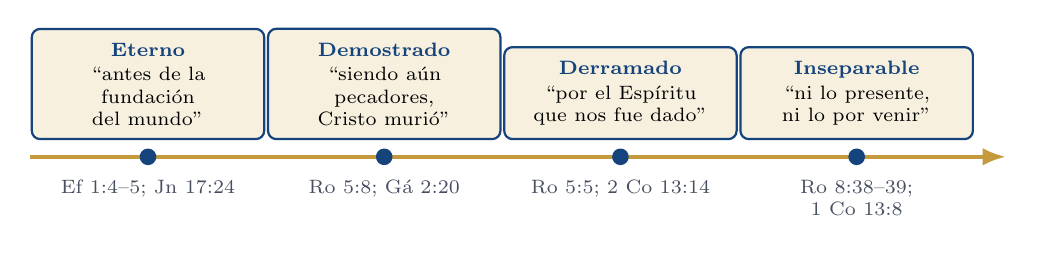
\begin{tikzpicture}[font=\small]
 \tikzset{hito/.style={caja,font=\scriptsize,text width=2.6cm,align=center}}
 \draw[-{Latex[length=3mm]},dorado,line width=1.6pt] (0,0) -- (12.4,0);
 \foreach \x/\t/\r/\p in {0.2/Eterno/{antes de la fundación del mundo}/{Ef 1:4--5; Jn 17:24},
                          3.2/Demostrado/{siendo aún pecadores, Cristo murió}/{Ro 5:8; Gá 2:20},
                          6.2/Derramado/{por el Espíritu que nos fue dado}/{Ro 5:5; 2 Co 13:14},
                          9.2/Inseparable/{ni lo presente, ni lo por venir}/{Ro 8:38--39; 1 Co 13:8}} {
   \fill[azul] (\x+1.3,0) circle (3pt);
   \node[hito,above=6pt] at (\x+1.3,0) {\textbf{\textcolor{azul}{\t}}\\[1pt]``\r''};
   \node[below=5pt,text width=2.6cm,align=center,font=\scriptsize\color{gris}] at (\x+1.3,0) {\p};
 }
\end{tikzpicture}\par\bigskip
\small El amor de Dios en Pablo: \destacar{eterno} en su origen, \destacar{soberano} en la cruz, \destacar{inmutable} en su final.\par
{\fontsize{5}{6}\selectfont\color{gris}\textit{Nota.} Elaboración propia.}
\end{frame}

\begin{frame}{``El cual me amó y se entregó a sí mismo por mí''}
\begin{cita}Con Cristo estoy juntamente crucificado, y ya no vivo yo, mas vive Cristo en mí; y lo que ahora vivo en la carne, lo vivo en la fe del Hijo de Dios, el cual me amó y se entregó a sí mismo por mí.\fuente{(Gá 2:20, RVR1960)}\end{cita}
\begin{columns}[t,onlytextwidth]
\begin{column}{0.49\textwidth}\scriptsize
\begin{itemize}
\item \grc{τοῦ ἀγαπήσαντός με}: aoristo singular. El perseguidor (Gá 1:13) se sabe amado en persona.
\item \grc{παραδόντος ἑαυτόν}: el amor no da algo, se da (cf. Ro 8:32).
\end{itemize}
\end{column}
\begin{column}{0.48\textwidth}
\begin{cita}Maridos, amad a vuestras mujeres, así como Cristo amó a la iglesia, y se entregó a sí mismo por ella.\fuente{(Ef 5:25, RVR1960)}\end{cita}
\precision{Ef 5 cita Gn 2:24, no Oseas; la relación con Os 3 es tipológica, apoyada en Ro 9:25.}
\end{column}
\end{columns}
\end{frame}

\begin{frame}{Los tres rasgos, de Israel a Pablo}
\scriptsize\renewcommand{\arraystretch}{1.2}
\begin{tabular}{@{}>{\RaggedRight\arraybackslash}p{1.8cm}>{\RaggedRight\arraybackslash}p{3.1cm}>{\RaggedRight\arraybackslash}p{3.1cm}>{\RaggedRight\arraybackslash}p{3.8cm}@{}}
\toprule
\textbf{Rasgo} & \textbf{Escrituras de Israel} & \textbf{Pablo} & \textbf{Lo que muestra la cruz} \\ \midrule
\destacar{Eterno} & Jer 31:3; Os 11:1 & Ef 1:4--5; 2 Ts 2:13, 16 & El Hijo amado desde antes de la fundación del mundo se entrega (Jn 17:24; Gá 2:20). \\
\destacar{Soberano} & Dt 7:7--8; 10:15; Mal 1:2; Os 14:4 & Ro 5:8; 9:13; Ef 2:4--5; Tit 3:4--5 & Cristo muere por débiles, impíos, pecadores y enemigos. \\
\destacar{Inmutable} & Mal 3:6; Os 11:8--9; Is 54:10; Cnt 8:7 & Ro 8:35--39; 1 Co 13:8 & Ni la muerte separa: el Amado resucitó e intercede (Ro 8:34). \\
\bottomrule
\end{tabular}\par\medskip
\begin{cita}Pero Dios, que es rico en misericordia, por su gran amor con que nos amó, aun estando nosotros muertos en pecados, nos dio vida juntamente con Cristo (por gracia sois salvos).\fuente{(Ef 2:4--5, RVR1960)}\end{cita}
\end{frame}

\begin{frame}{La plenitud del amor en Cristo}
\begin{cita}\ldots{} a fin de que, arraigados y cimentados en amor, seáis plenamente capaces de comprender con todos los santos cuál sea la anchura, la longitud, la profundidad y la altura, y de conocer el amor de Cristo, que excede a todo conocimiento, para que seáis llenos de toda la plenitud de Dios.\fuente{(Ef 3:17--19, RVR1960)}\end{cita}
\begin{cita}Porque en él habita corporalmente toda la plenitud de la Deidad.\fuente{(Col 2:9, RVR1960)}\end{cita}
\small El amor que Dios es se ve entero en el Hijo: el Padre ama al Hijo desde siempre y en él ama a los suyos ``como también a mí me has amado'' (Jn 17:23). Pink lo llama amor ``infinito'' (Pink, 2020, p.~86).
\end{frame}

% ------------------------------------------------------------------
\section{Aplicación}

\begin{frame}{Del amor de Dios al amor del creyente}
\small\renewcommand{\arraystretch}{1.25}
\begin{tabular}{@{}>{\RaggedRight\arraybackslash}p{2.0cm}>{\RaggedRight\arraybackslash}p{4.4cm}>{\RaggedRight\arraybackslash}p{5.4cm}@{}}
\toprule
\textbf{Rasgo} & \textbf{En Dios} & \textbf{Reflejo en el creyente} \\ \midrule
\destacar{Eterno} & Amó antes de que existiéramos (Jer 31:3; Ef 1:4) & \textbf{Seguridad} sin temor: ``el perfecto amor echa fuera el temor'' (1 Jn 4:18--19) \\
\destacar{Soberano} & Amó sin causa en nosotros (Dt 7:7--8; Ro 5:8) & \textbf{Humildad}: ``¿qué tienes que no hayas recibido?'' (1 Co 4:7); amar al que no lo merece (Dt 10:19; Mt 5:44) \\
\destacar{Inmutable} & No deja de amar (Mal 3:6; Ro 8:39) & \textbf{Perseverancia}: ``¿quién nos separará?'' (Ro 8:35); ``conservaos en el amor de Dios'' (Jud 21) \\
\bottomrule
\end{tabular}\par\medskip
\begin{cita}Amados, si Dios nos ha amado así, debemos también nosotros amarnos unos a otros.\fuente{(1 Jn 4:11, RVR1960)}\end{cita}
\end{frame}

\begin{frame}{Amar como él}
\begin{columns}[t,onlytextwidth]
\begin{column}{0.49\textwidth}
\begin{cita}\ldots{} que ama también al extranjero dándole pan y vestido. Amaréis, pues, al extranjero; porque extranjeros fuisteis en la tierra de Egipto.\fuente{(Dt 10:18--19, RVR1960)}\end{cita}
\begin{cita}Sed, pues, imitadores de Dios como hijos amados. Y andad en amor, como también Cristo nos amó, y se entregó a sí mismo por nosotros\ldots\fuente{(Ef 5:1--2, RVR1960)}\end{cita}
\end{column}
\begin{column}{0.48\textwidth}
\begin{cita}El amor no hace mal al prójimo; así que el cumplimiento de la ley es el amor.\fuente{(Ro 13:10, RVR1960; cf. Lv 19:18)}\end{cita}
\begin{cita}Todo lo sufre, todo lo cree, todo lo espera, todo lo soporta. El amor nunca deja de ser\ldots\fuente{(1 Co 13:7--8, RVR1960)}\end{cita}
\scriptsize\grc{ἡ ἀγάπη οὐδέποτε πίπτει}: lo que Malaquías dijo de Dios (``no cambio''), Pablo lo dice del amor.
\end{column}
\end{columns}
\end{frame}

\begin{frame}{Conclusión}
\begin{tcolorbox}[colback=papiro,colframe=dorado,boxrule=1.2pt,arc=3pt]
\small Conocer a Dios como amor no es conocer un sentimiento, sino a una persona que ama \destacar{desde siempre}, \destacar{sin causa fuera de sí} y \destacar{sin cambio}. Ese amor se dejó ver en Moriah, en el Sinaí, en la casa de Oseas y, por último, en la cruz, donde el Padre ``no escatimó ni a su propio Hijo'' (Ro 8:32).
\end{tcolorbox}
\begin{cita}Y nosotros hemos conocido y creído el amor que Dios tiene para con nosotros. Dios es amor; y el que permanece en amor, permanece en Dios, y Dios en él.\fuente{(1 Jn 4:16, RVR1960)}\end{cita}
\end{frame}

% ------------------------------------------------------------------
\section{Glosario}

\begin{frame}{Glosario}
\scriptsize
\begin{columns}[t,onlytextwidth]
\begin{column}{0.49\textwidth}
\begin{description}\setlength{\itemsep}{1pt}
\item[\emph{Agápē}] (\grc{ἀγάπη}) amor; \emph{agapáō}, amar.
\item[\emph{Ahav}] (\heb{אָהַב}) amar; \emph{ahavá}, amor.
\item[\emph{Ahavat olam}] (\heb{אַהֲבַת עוֹלָם}) amor eterno (Jer 31:3).
\item[\emph{Hafaj}] (\heb{הָפַךְ}) trastornar, dar vuelta (Os 11:8).
\item[\emph{Hilasmós}] (\grc{ἱλασμός}) propiciación (1 Jn 4:10).
\item[\emph{Jashaq}] (\heb{חָשַׁק}) ligarse por amor (Dt 7:7).
\item[\emph{Javiv}] (\heb{חָבִיב}) amado, querido (Avot 3:14).
\item[\emph{Mashaj}] (\heb{מָשַׁךְ}) atraer, prolongar (Jer 31:3).
\end{description}
\end{column}
\begin{column}{0.49\textwidth}
\begin{description}\setlength{\itemsep}{1pt}
\item[\emph{Nedavá}] (\heb{נְדָבָה}) ofrenda voluntaria; ``de pura gracia''.
\item[\emph{Philéō}] (\grc{φιλέω}) querer, tener afecto.
\item[\emph{Rajam}] (\heb{רָחַם}) amar entrañablemente; arameo ``amar''.
\item[Shemá] (\heb{שְׁמַע}) ``Oye'' (Dt 6:4--9).
\item[\emph{Synístēmi}] (\grc{συνίστημι}) demostrar (Ro 5:8).
\item[\emph{Yedid}] (\heb{יְדִיד}) amado (Jedidías, 2 S 12:25).
\item[\emph{Yajid}] (\heb{יָחִיד}) único (Gn 22:2).
\item[\emph{Jorízō}] (\grc{χωρίζω}) separar (Ro 8:35, 39).
\end{description}
\end{column}
\end{columns}
\end{frame}

% ------------------------------------------------------------------
\section{Referencias}

\begin{frame}{Referencias}
\fontsize{5.1}{6.1}\selectfont
\begin{columns}[t,onlytextwidth]
\begin{column}{0.49\textwidth}
\refapa{Carson, D.~A. (2000). \emph{The difficult doctrine of the love of God}. Crossway.}
\refapa{Carson, D.~A. (2013). \emph{Falacias exegéticas}. Editorial CLIE.}
\refapa{Dunn, J.~D.~G. (1998). \emph{The theology of Paul the apostle}. Eerdmans.}
\refapa{Elliger, K., \& Rudolph, W. (Eds.). (1997). \emph{Biblia Hebraica Stuttgartensia} (5.ª ed.). Deutsche Bibelgesellschaft.}
\refapa{García Martínez, F. (1992). \emph{Textos de Qumrán}. Trotta.}
\refapa{Maimónides. (s.f.). \emph{Mishné Torá: Hiljot Teshuvá} [10:3]. Sefaria.}
\refapa{\emph{Misná: Berajot} [9:5]; \emph{Yadayim} [3:5]; \emph{Pirké Avot} [3:14; 5:16]. (s.f.). Sefaria.}
\refapa{Moo, D.~J. (1996). \emph{The epistle to the Romans}. Eerdmans.}
\refapa{Moran, W.~L. (1963). The ancient Near Eastern background of the love of God in Deuteronomy. \emph{Catholic Biblical Quarterly}, \emph{25}(1), 77--87.}
\refapa{Nestle, E., \& Aland, K. (2012). \emph{Novum Testamentum Graece} (28.ª ed.). Deutsche Bibelgesellschaft.}
\refapa{Pink, A.~W. (2020). \emph{Los atributos de Dios} (E. Rodríguez Cruz, Trad.). Chapel Library. (Obra original publicada en 1930)}
\end{column}
\begin{column}{0.49\textwidth}
\refapa{Rahlfs, A., \& Hanhart, R. (Eds.). (2006). \emph{Septuaginta}. Deutsche Bibelgesellschaft.}
\refapa{Rashi. (s.f.). \emph{Comentario a la Torá} [Dt 7:7] y \emph{al Cantar de los Cantares}. Sefaria.}
\refapa{\emph{Santa Biblia: Reina-Valera 1960}. (1960). Sociedades Bíblicas en América Latina.}
\refapa{\emph{Shemot Rabá} [3:6]. (s.f.). Sefaria.}
\refapa{\emph{Sidur asquenazí: Ahavá rabbá; Ahavat olam}. (s.f.). Sefaria.}
\refapa{\emph{Sifré Devarim} [32]. (s.f.). Sefaria.}
\refapa{Steinsaltz, A. (Ed.). (2017). \emph{Koren Talmud Bavli} [Berajot 11b, 61b; Julín 89a]. Sefaria.}
\refapa{Strong, J. (1890). \emph{The exhaustive concordance of the Bible}. Hunt \& Eaton.}
\refapa{\emph{Targum Ónkelos} [Dt 6:5]. (s.f.). Sefaria.}
\refapa{Vermes, G. (2004). \emph{The complete Dead Sea Scrolls in English}. Penguin.}
\refapa{Vine, W.~E. (1999). \emph{Diccionario expositivo de palabras del Antiguo y del Nuevo Testamento exhaustivo}. Caribe.}
\end{column}
\end{columns}
\par\smallskip{\color{gris}Citas bíblicas: RVR1960; ``Jehová'' se reemplaza por \SENOR. Hebreo: BHS; griego: NA28 y LXX. Lo rabínico y lo interpretativo se marca como \emph{precisión}.}
\end{frame}

\end{document}
